\section{Imagen}
\label{sec:imagen}

Imagen \cite{imagen} is a T2I diffusion model that builds on the power of large transformer language models \cite{transformer} (LLMs) to generate high-fidelity images. The combination of diffusion and LLMs have shown remarkable outputs. 

The paper has 5 main key takeaways and observations:

\begin{enumerate}
    \item \textbf{Effectiveness of large frozen text encoders}: one of the main observation in the paper that a large frozen language model trained only on text data have a significant impact on the fidelity of generated images compared to increasing the parameters of the diffusion image model. Scaling the language model is easy, since unlabeled text data is abundant and available on the internet.
    \item \textbf{Dynamic thresholding}: is a new sampling technique (section \ref{subsec:imagen_diffusion_guidance_weight}) that improves image fidelity and text-image alignment, which improves upon static thresholding.
    \item \textbf{Effective U-Net}: a new U-Net architecture that is simpler and more memory efficient.
    \item \textbf{COCO FID score of 7.27}: imagen achieved a new state-of-the-art COCO FID score of 7.27, which outperforms all other previous works.
    \item \textbf{DrawBench}: a new human evaluation benchmark for T2I task. Imagen outperforms all other works, including DALL-E \cite{dalle}, VQ-GAN+CLIP \cite{vqgan_clip}, LDM \cite{stable_diffusion}, GLIDE \cite{glide}, and DALL-E 2 \cite{dalle_2}.
\end{enumerate}



















\subsection{Text-to-Text Transfer Transformer (T5)}
\label{subsec:t5}

\textbf{T}ext-\textbf{t}o-\textbf{T}ext \textbf{T}ransfer \textbf{T}ransformer (T5) \cite{t5_model} by Google Research is a language model that treats tasks as a text-to-text (T2T) problems. For example we could prompt the model:

\begin{itemize}
    \item \textbf{Summarization}: "Translate the following text to a summary: ..."
    \item \textbf{Translation}: "Translate the following text from English to French: ..."
    \item \textbf{Text classification}: "Classify the following text into one of the following categories: ..."
    \item \textbf{Question answering}: "Answer the following question: ..."
\end{itemize}

as well as other T2T tasks. In short, this knowledge can be viewed as developing a 'general-purpose' model that can understand text, instead of explicitly training the model to complete the specific downstream task.

The T5 model is open-source and was trained on large corpora of textual data. The base version of the model (T5-base) consists of 220 million parameters, while the largest version of the model (T5-XXL) consists of \textbf{11 billion parameters}. In the context of Imagen, \textbf{the Imagen model uses a frozen version of T5-XXL model} to encode conditional text prompts.

\textbf{Pre-training}: Unsupervised learning is appealing because unlabeled text data is abundant and available on the Internet. For example, the Common Crawl project \cite{common_crawl_project} is a non-profit organization that crawls the internet and provides free access to its achieved datasets to the public. A lot of research has been done on LLM models on large scale datasets, and the consensus is that \textbf{the larger the dataset, the better the model performs} \cite{radford2019language} \cite{jozefowicz2016exploring} \cite{hestness2017deep}. The T5 models were trained on the "Colossal Clean Crawled Corpus" (C4) dataset, which consists of 750GB of English text data scraped from the web.

\textbf{The training objective} of T5 model is called \textbf{span corruption}, which is stronger version of \textbf{masked language modeling}. Given a sentence, some words and some contiguous words are masked (in masked language modeling, only single words are masked), and the model should predict those words. For example: "Thank you for inviting me to your party last week", where the masked words are "for inviting" and "last". And the model should predict those words in the following sentence: "Thank you [MASKED] me to your party [MASKED] week". The model should learn to reconstruct the missing tokens.

\begin{figure}[h]
    \centering
    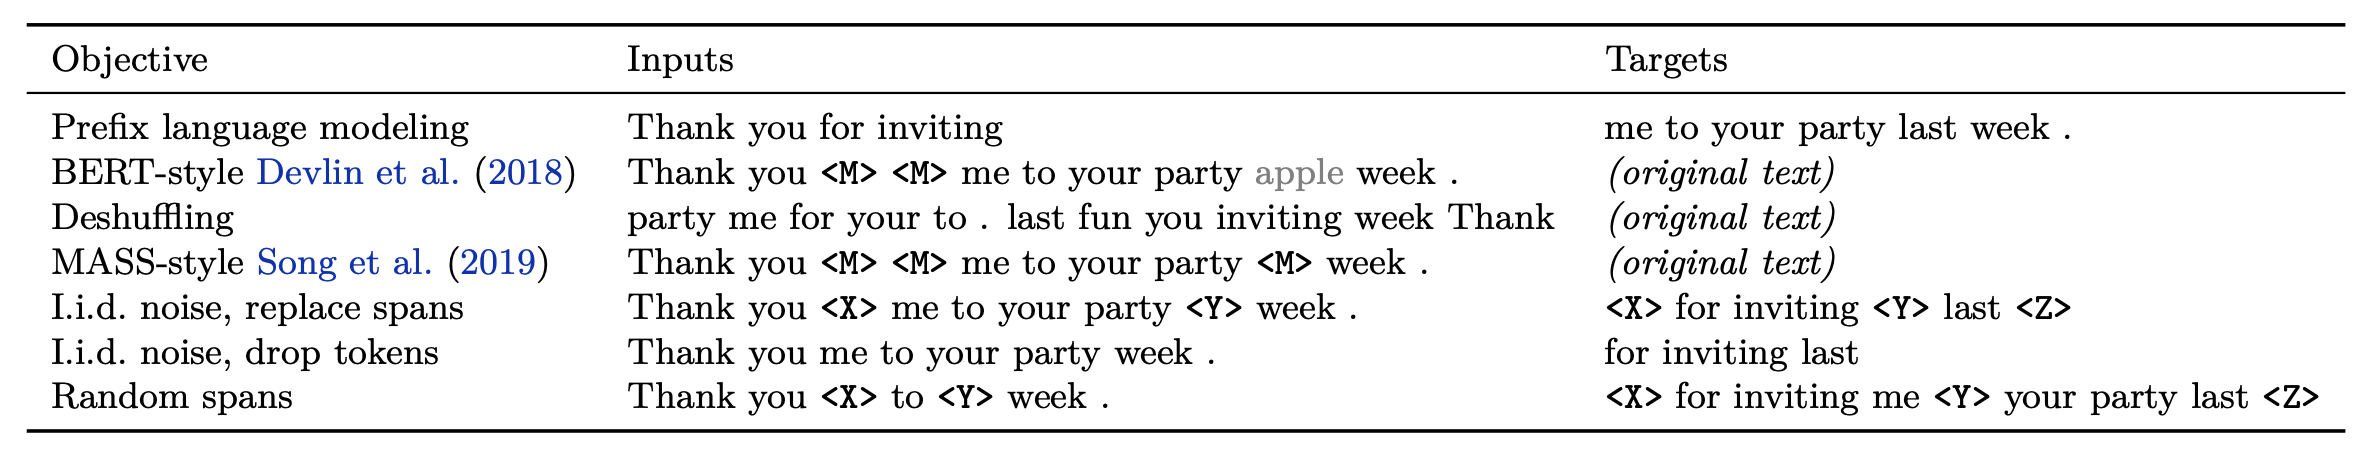
\includegraphics[width=1\textwidth]{images/imagen/t5_objectives.png}
    \caption{Mask modeling in T5 \cite{t5_model}.}
    \label{fig:t5_objectives}
\end{figure}

In figure \ref{fig:t5_objectives} \textless M\textgreater\ denotes shared mask token (the same mask token is used to represent all masked positions in the input). \textless X\textgreater, \textless Y\textgreater, and \textless Z\textgreater\ denote sentinel tokens which have unique token IDs; they mark specific masked positions that the model should reconstruct.















\subsection{Pre-trained text encoders}

In Imagen \cite{imagen} the researchers explored some of the biggest and most advanced text encoders: \textbf{T5-XXL} \cite{t5_model}, \textbf{GPT} \cite{gpt} \cite{mingpt} \cite{gpt_another}, and \textbf{BERT} \cite{bert}. These LLMs were trained exclusively on text datasets, which are substantially larger compared to image-text pair datasets (as used in models like \textbf{CLIP}).

Freezing these models \footnote{When we freeze models we generally mean that some (or all) of the parameters of the model are not changed during training. How? When a layer is frozen during training, no gradient updates will occur for this layer. Gradients will still flow from frozen layer to non-frozen layer, it doesn't skip the backpropagation. It just passes the gradients from the next layer to the previous layer.} provides significant advantage over training them: less memory and compute costs.














\subsection{Diffusion guidance weight}
\label{subsec:imagen_diffusion_guidance_weight}

As described before (section \ref{subsec:classifier_free_diffusion_guidance}), there are two methods to increase sample quality with the tradeoff of diversity:

\begin{itemize}
    \item \textbf{Classifier guidance} uses a separate, pre-trained classifier model to guide the image generation process in diffusion models by adjusting the noise based on how closely the generated image matches a desired condition.
    
    \item \textbf{Classifier-free guidance} (CFG) removes the need for a separate classifier by training the diffusion model itself to optionally condition on the label or text input.
\end{itemize}

More formally, in CFG, sampling is performed weighting the conditional and unconditional signals:

\begin{equation}
    \underbrace{\tilde{\epsilon}_\theta (z_t, c)}_{\text{adj noise prediction}} = \underbrace{w \epsilon_\theta (z_t, c)}_{\text{conditional score}} + \underbrace{(1 - w) \epsilon_\theta (z_t)}_{\text{unconditional score}}
    \label{eq:classifier_free_guidance}
\end{equation}

where $\epsilon_\theta$ is the noise prediction with the learned parameters $\theta$, $w$ is the guidance weight, $c$ is the condition, and $z_t$ is the latent variable at timestep $t$.

Imagen depends on CFG for effective text conditioning. They found that increasing the guidance weight improves image-text alignment but reduces image fidelity. Its caused by \textbf{train-test mismatch}: looking at equation \ref{eq:classifier_free_guidance} if we set $w$ to 1, then we disable CFG, and then the model won't be trained on unconditional samples (only on conditional signals). This causes the model to generate outputs that exceed the noise prediction in the normalized range of [-1, 1]. And when iteratively applying the model to its own outputs at each step, errors caused by this mismatch accumulate, which causes unnatural artifacts in output images. When we set $w>1$ then it improves the model's image-text alignment, but damages image fidelity.

For this reason they investigated static thresholding and dynamic thresholding:

\textbf{Static thresholding} applies the clipping operation to force the $x$-prediction output to fit to the normalized range of [-1, 1]. However, static thresholding still result in over-saturated and less detailed images as the guidance weight approaches 1.

\textbf{Dynamic thresholding}: instead of clipping the $x$-prediction to the normalized range, it sets a dynamic threshold $s$ based on the distribution of absolute pixel values in the current $x$-prediction, allowing the threshold to adapt to the specific output of the model at that moment. In other words, if the pixel values are saturated (close to the [-1, 1] range), dynamic thresholding pushes them inwards by thresholding in the range [-$s$, $s$] and then dividing by $s$.

\begin{figure}
    \centering
    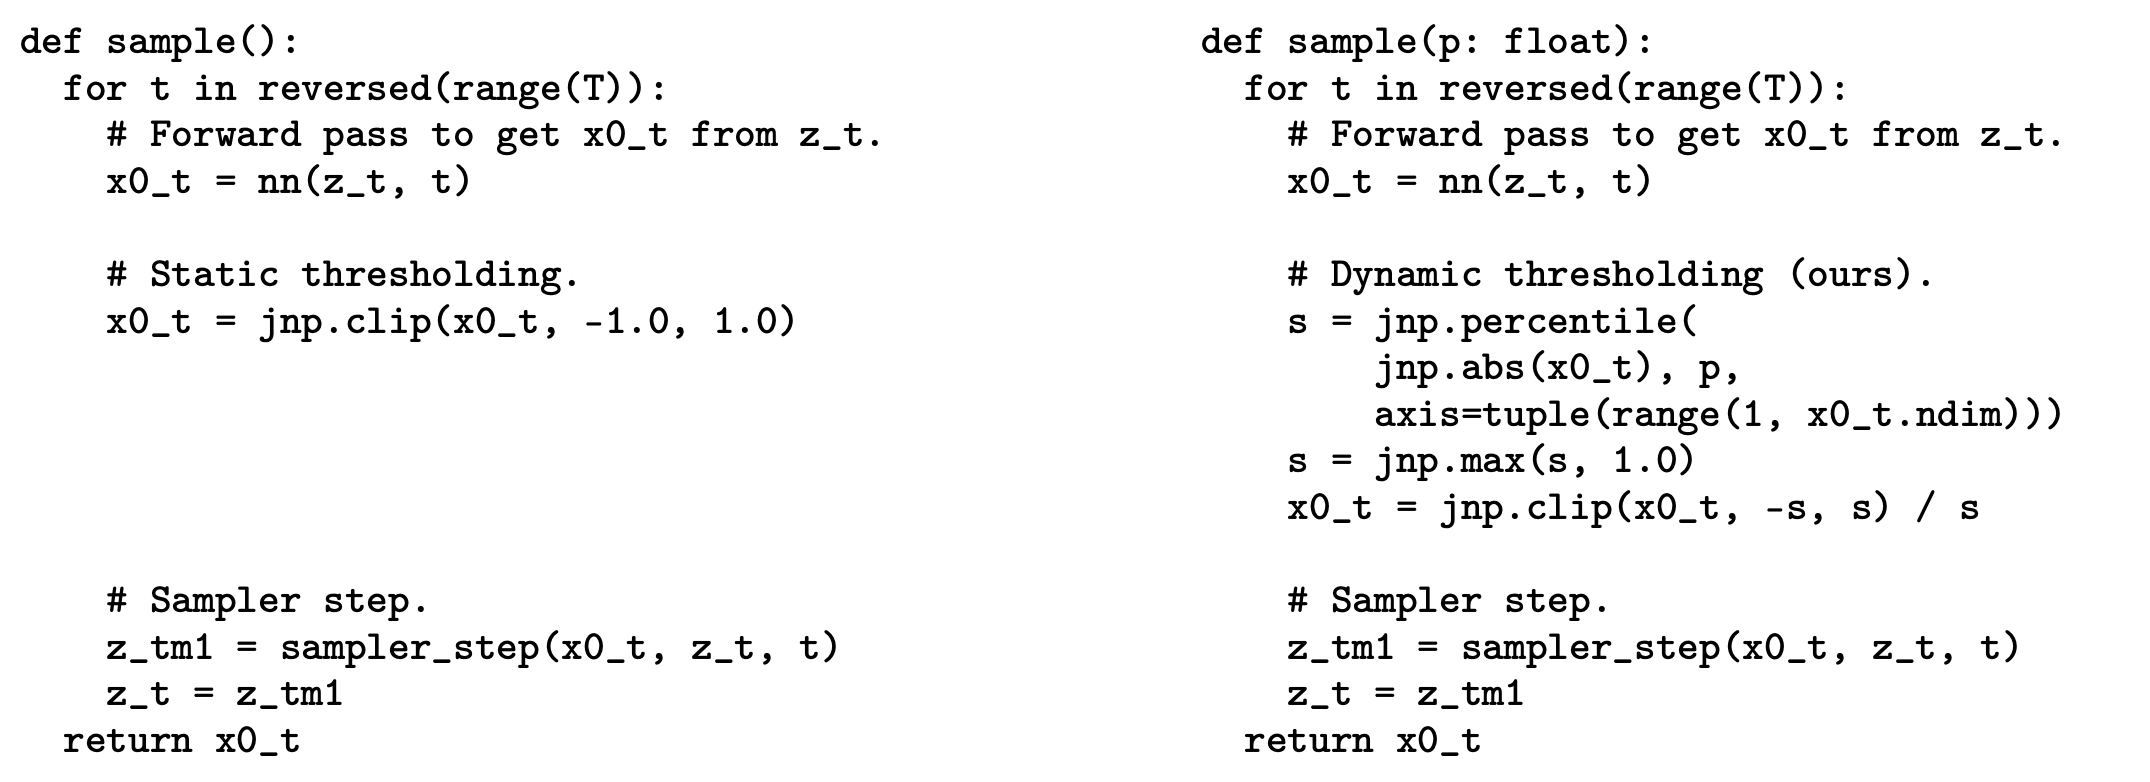
\includegraphics[width=0.7\textwidth]{images/imagen/static_dynamic_thresholding.png}
    \caption{Static (left) and dynamic (right) thresholding code implementation \cite{imagen}.}
    \label{fig:imagen_dynamic_thresholding}
\end{figure}

\begin{figure}
    \centering
    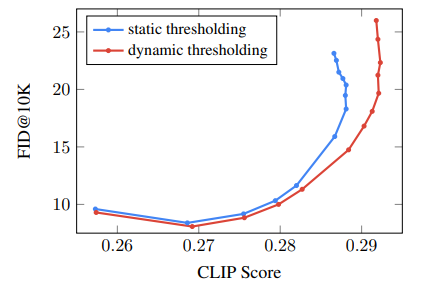
\includegraphics[width=0.4\textwidth]{images/imagen/static_vs_dynamic_thresholding.png}
    \caption{Static vs dynamic thresholding \cite{imagen}.}
    \label{fig:imagen_static_vs_dynamic_thresholding}
\end{figure}

The implementation of static and dynamic thresholding is shown in figure \ref{fig:imagen_dynamic_thresholding}. The impact of dynamic thresholding is shown in figure \ref{fig:imagen_static_vs_dynamic_thresholding} where its shown that dynamic thresholding produces samples with higher image-text alignment (CLIP) and fidelity (FID) compared to static thresholding.
















\subsection{Super-resolution via Repeated Refinement (SR3)}

\label{subsec:imagen_sr3}

In a 2021 paper \cite{sr3}, the Google Research team introduced a new super-resolution model based on diffusion process. \textbf{S}uper-resolution via \textbf{R}epeated \textbf{R}efinment (SR3) model upsamples in iterative manner, similar to reverse diffusion. It upsamples images from $64\times 64$ to $256\times 256$ and finally to $1024\times 1024$.

SR3 achieves close to a 50\% fool rate (47\%) \footnote{A 50\% fool rate means humans can't distinguish between a generated face image and an image of a real face.} on $16\times 16 \rightarrow 128\times 128$ faces, outperforming the previous state-of-the-art GAN models (FSRGAN and PULSE).

\textbf{Iterative refinement}: Given low-resolution image $x_{low}$ the model applies \textbf{bicubic interpolation} \footnote{Bicubic interpolation is a method for resizing images that uses the closest 4x4 pixels grid to estimate new values, resulting in smoother transitions (compared to nearest-neighbor or bilinear interpolation) and fewer visual artifacts.} to upscale the image to the target resolution to get high-resolution image $x$ and then concatenates $x$ with pure Gaussian noise $y_t \sim \mathcal{N} (0, I)$ channel-wise (see figure \ref{fig:sr3_architecture}). Then the U-Net iteratively refines the image $(x, y_t)$ by denoising. The output of a single refinement step (from the U-Net) is $y_{t-1}$. Then in the next refinement step, $x$ is concatenated with $y_{t-1}$ and the process is repeated until we reach $y_0$. The final output is a high-resolution image $y_0$. Note that both $x$ (after the upsampling), $y_i$ are all on same resolution / dimension (see figure \ref{fig:sr3_architecture}).

\textbf{The architecture of SR3} modified the diffusion U-Net: they replaced the original DDPM residual blocks with residual blocks from BigGAN \cite{biggan_deep}, rescaled skip connections by $\frac{1}{\sqrt{2}}$, increased the number of residual blocks, and increased the number of the channel multipliers \footnote{Channel multipliers in a U-Net are the scaling factors used to adjust the number of feature channels at different U-Net layers. In other words, they increased the depth of the features at the cost of decreasing resolution at the convolution layers (down convolution, up convolution layers)} at different resolutions.

% \begin{table}[h!]
%     \centering
%     \begin{tabular}{|l|m{8cm}|}
%         \hline
%         \textbf{Prior to Super Resolution} & \textbf{Limitations} \\ \hline
%         Autoregressive Models           & Computationally expensive; Limited resolution \\ \hline
%         Variational Autoencoder         & Sub-optimal sample quality \\ \hline
%         Generative Adversarial Network  & Difficult to optimize; Requires additional functions to prevent instability \\ \hline
%     \end{tabular}
%     \caption{Related works to super-resolution to SR3 and their limitations compared to SR3.}
% \end{table}


\begin{figure}
    \centering
    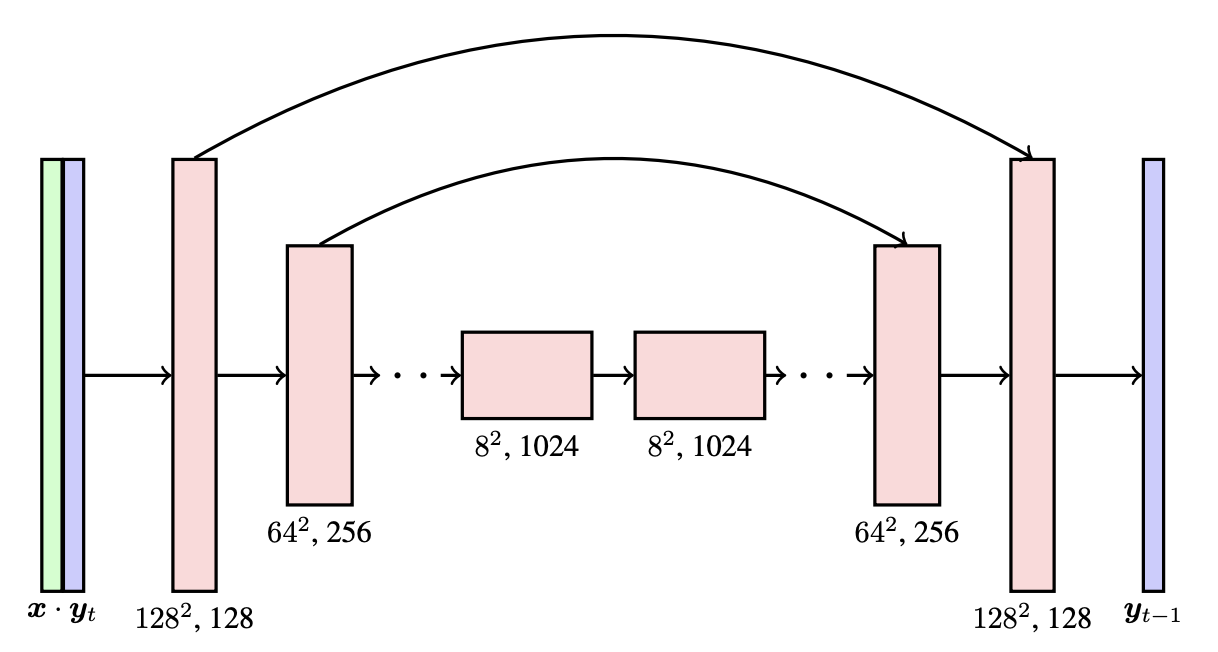
\includegraphics[width=0.5\textwidth]{images/imagen/sr3_architecture.png}
    \caption{SR3 $16\times 16 \rightarrow 128\times 128$ upsampling where $x$ is the input image, upscaled to the target resolution using bicubic interpolation, and then its concatenated with the noise $y$ \cite{sr3}.}
    \label{fig:sr3_architecture}
\end{figure}















\subsection{Cascaded diffusion models (CDMs)}

Cascaded diffusion models, introduced in a 2022 paper \cite{cascaded_diffusion_models} by Google Research, builds upon the SR3 paper \cite{sr3} and introduces a new method for super-resolution (SR) called Cascaded Diffusion Models (CDMs). CDMs use a base diffusion model that output image at low resolution, followed by a sequence (pipeline) of SR3 SR diffusion models that progressively upsamples until we reach the target resolution.

The CDM paper \cite{cascaded_diffusion_models} outperformed VQ-VAE 2 \cite{vqvae2} and BigGAN-deep \cite{biggan_deep} in SR task in FID metric on ImageNet dataset.

A big strength of CDMs is the ability to train and fine tune each model individually.

\textbf{Conditioning augmentation} is the main and critical part of the paper \cite{cascaded_diffusion_models}, which allows generating images with higher FID, compared to without conditioning augmentation. Conditioning augmentation involves using data augmentation techniques on the low-resolution input image for each SR model in the cascaded pipeline. Augmentations such as Gaussian noise and Gaussian blur are applied to the image which helps prevent each SR model from overfitting to the low-resolution input.

\begin{figure}
    \centering
    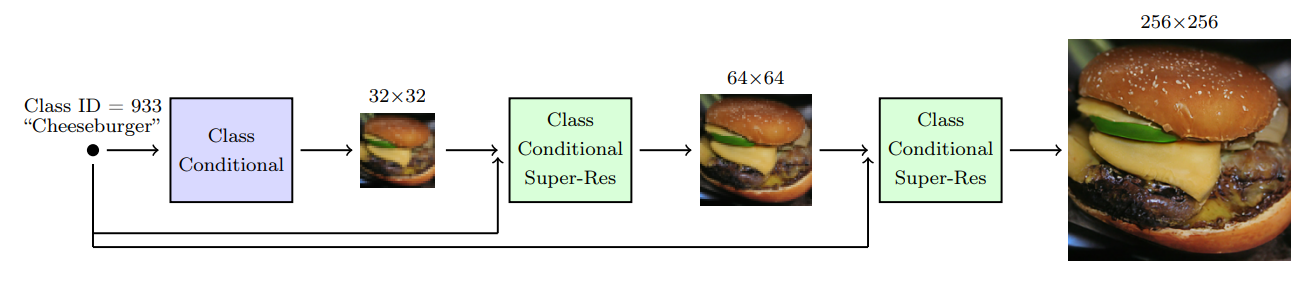
\includegraphics[width=0.7\textwidth]{images/imagen/cdm_architecture.png}
    \caption{CDM upsamples low-resolution image in the pipeline, conditioned on labels \cite{cascaded_diffusion_models}.}
    \label{fig:imagen_cdm_architecture}
\end{figure}

In figure \ref{fig:imagen_cdm_architecture} we see CDM upsamples the low-resolution image in multiple steps with class conditional super-resolution; the condition is class ID = "Cheeseburger" which guides the generation pipeline to upsample correctly.























\subsection{Architecture}

An overview of Imagen architecture is shown in figure \ref{fig:imagen_architecture}.

The researchers conducted experiments with frozen LLMs such as BERT \cite{bert}, T5 \cite{t5_model}, and CLIP \cite{openai_clip} and found that humans prefer T5-XXL over CLIP. T5-XXL (T5-Extra Extra Large) text encoder maps text prompts to embeddings. The T5-XXL model has 11 billion parameters, and its the largest version of the T5 model. All the diffusion models are conditioned on the same text embeddings.

\textbf{Base model}: the base model is a $64\times 64$ T2I diffusion model. The network is conditioned on text embeddings (via cross-attention and layer normalization layers), as well as with diffusion timestep embeddings, similar to the class embedding conditioning in the CDM paper \cite{cascaded_diffusion_models}.

\textbf{SR models}: they used modified U-Net based on the improved DDPM paper \cite{openai_improved_ddpm} by OpenAI, By improving the U-Net they achieved 2-3x faster inference and convergence speed; they call this variant "\textbf{Efficient U-Net}". For the $256\times 256 \rightarrow 1024\times 1024$ SR model, they removed self-attention layers but keep the cross-attention layers.

\textbf{Efficient U-Net}: is a new U-Net architectural variant for SR models. Its more memory efficient and \textbf{2-3x faster in training and inference time}. There are several modifications to the U-Net architecture:

\begin{enumerate}
    \item \textbf{More residual blocks}: adding more residual blocks for lower resolutions, since lower-resolution images typically have more channels. They used 8 residual blocks at lower-resolution compared to typical 2-3 residual blocks used in a standard U-Net.
    \item \textbf{Scaling the skip connections} by $\frac{1}{\sqrt{2}}$, similar to SR3 \cite{sr3}, significantly improves convergence speed.
    \item \textbf{Reversing order of downsampling and upsampling blocks}: In a standard U-Net downsampling block, downsampling occurs after the convolution layers, and in the upsampling block, upsampling is done before the convolutions. They reverse this order for both blocks which significantly improves the forward pass without performance degradation.
\end{enumerate}

The efficient U-Net architecture for $64\times 64 \rightarrow 256\times 256$ is shown in figure \ref{fig:imagen_efficient_unet}.

\begin{figure}
    \centering
    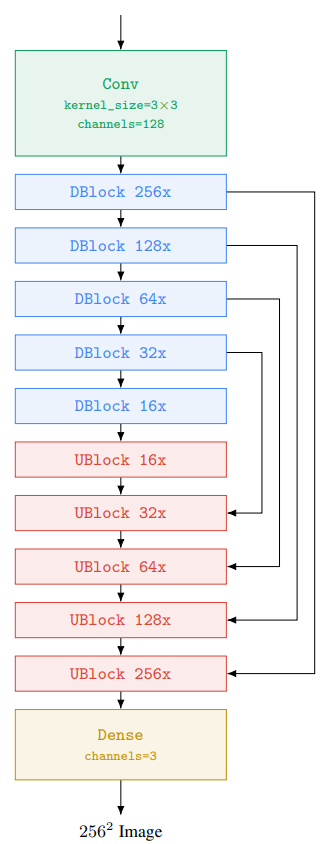
\includegraphics[width=0.25\textwidth]{images/imagen/efficient_unet.png}
    \caption{Efficient U-Net architecture for $64\times 64 \rightarrow 256\times 256$ SR model, proposed in Imagen \cite{imagen}.}
    \label{fig:imagen_efficient_unet}
\end{figure}

Similar to LDMs, Imagen also uses CFG \cite{classifier_free_guidance} (section \ref{subsec:classifier_free_diffusion_guidance}). Imagen depends critically on CFG for effective text conditioning.

\begin{figure}
    \centering
    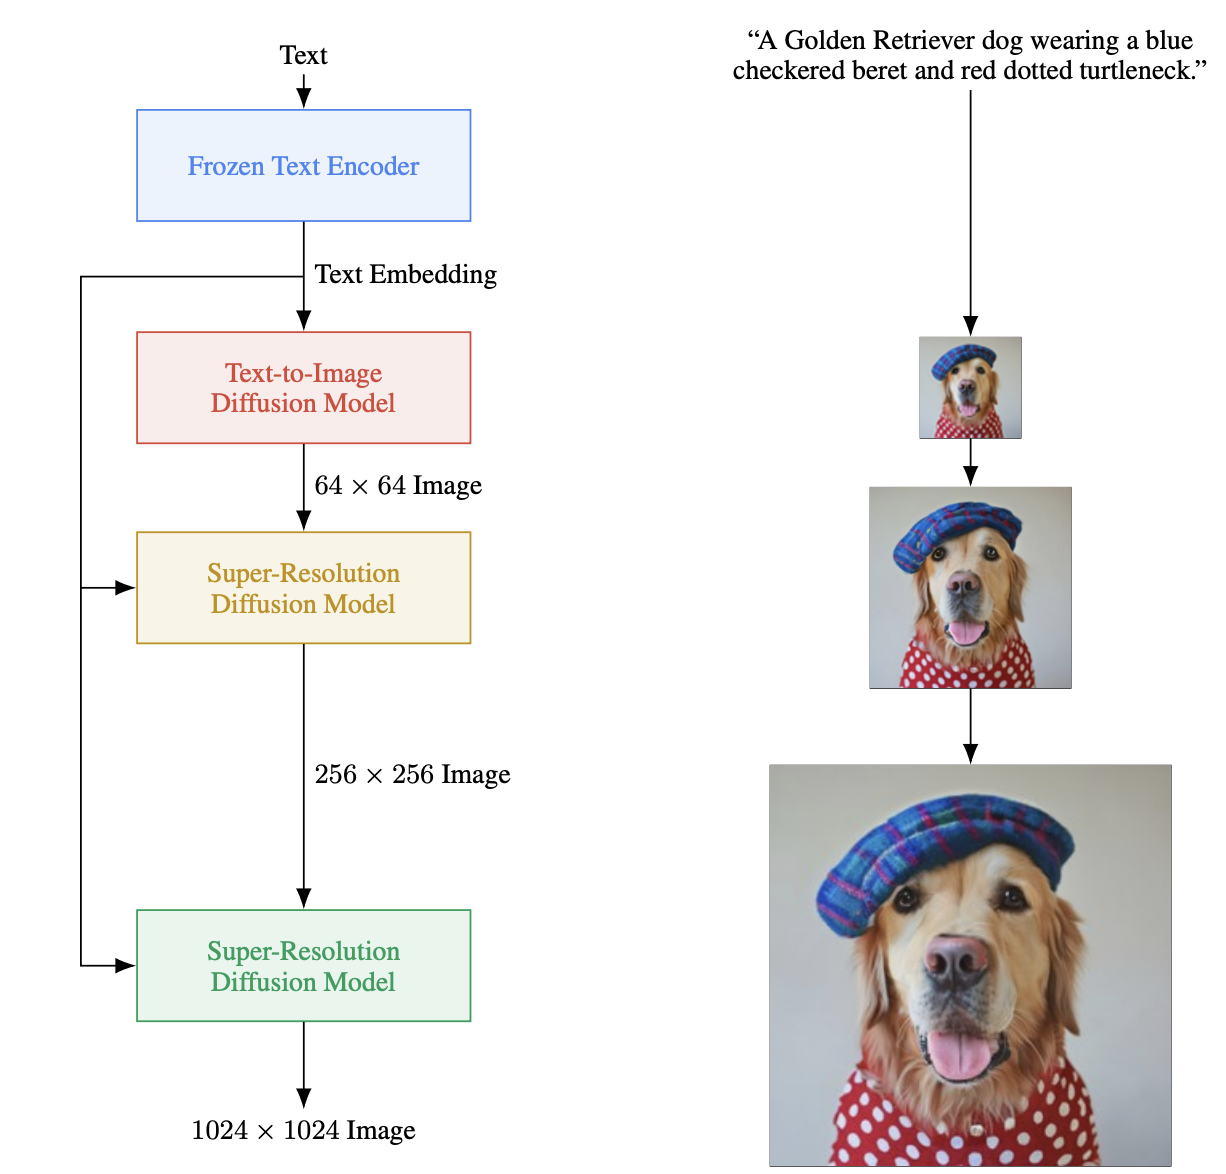
\includegraphics[width=0.5\textwidth]{images/imagen/architecture.png}
    \caption{Overview of Imagen architecture \cite{imagen}.}
    \label{fig:imagen_architecture}
\end{figure}

\textbf{Noise conditioning}: Imagen corrupts the $64\times 64$ image with Gaussian noise. The amount of noise is random at training but arbitrary at inference time. They control the amount of corruption with \textit{aug\_level}, and the SR model is conditioned on the augmentation level.

\textbf{Number of parameters}: the base T2I diffusion $64\times 64$ model has 2 billion parameters. The $64\times 64 \rightarrow 256\times 256$ SR model has 600 million parameters, and the $256\times 256 \rightarrow 1024\times 1024$ SR model has 400 million parameters. The size of the T5-XXL text encoder is 4.6 billion parameters.

\begin{figure}
    \centering
    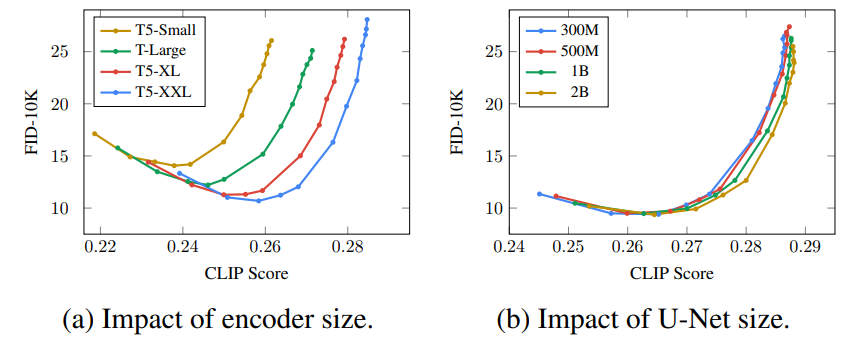
\includegraphics[width=0.75\textwidth]{images/imagen/encoder_vs_unet_size_impact.png}
    \caption{Scaling the encoder size is more impactful than scaling the U-Net size \cite{imagen}.}
    \label{fig:imagen_scaling_encoder_more_impactful_than_unet_scaling}
\end{figure}

\textbf{Scaling text encoder size is more important than U-Net size}: the researchers found that scaling the text encoder has significantly more impact than increasing U-Net size: see figure \ref{fig:imagen_scaling_encoder_more_impactful_than_unet_scaling}.



% DBlock, UBlock

\begin{figure}
    \centering
    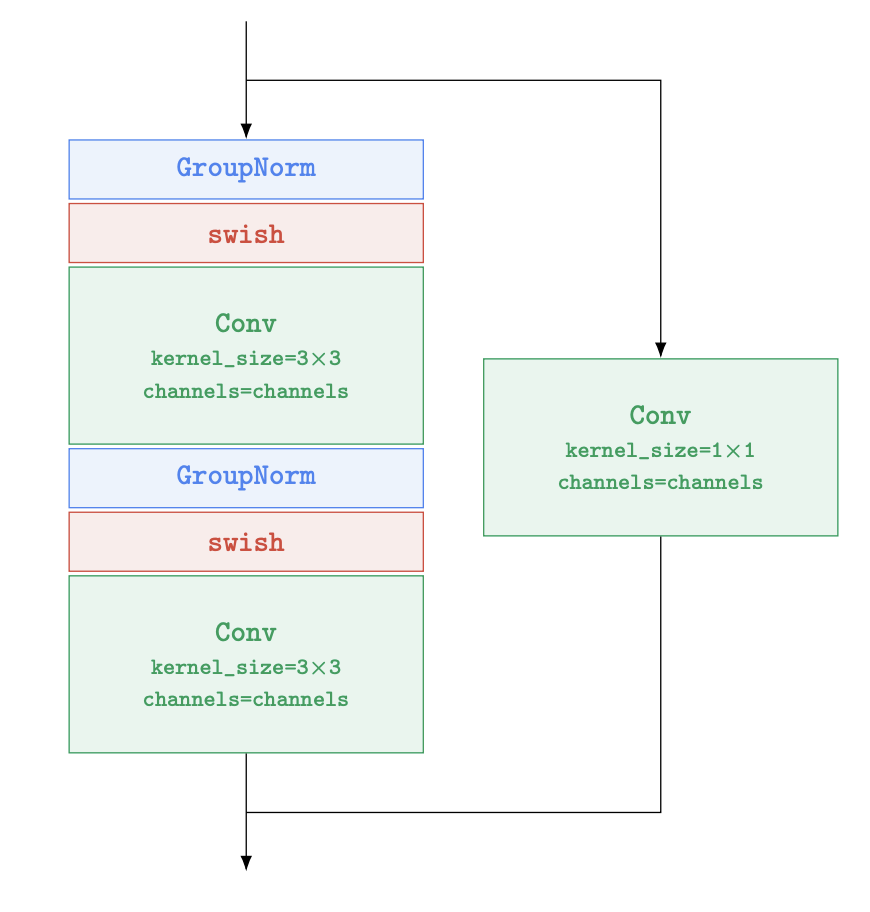
\includegraphics[width=0.35\textwidth]{images/appendix/imagen/unet_resnetblock.png}
    \caption{Imagen efficient U-Net \texttt{ResNetBlock} architecture \cite{imagen}.}
    \label{fig:imagen_resnetblock}
\end{figure}

In figure \ref{fig:imagen_resnetblock} we can see the \texttt{ResNetBlock} which is in use by both the \texttt{DBlock} and the \texttt{UBlock}. The only input of the \texttt{ResNetBlock} is the number of channels. The activation function is Swish (equation \ref{eq:appendix_activations_swish}). 

\begin{figure*}
    \centering
    \begin{subfigure}[b]{0.5\textwidth}   
        \centering 
        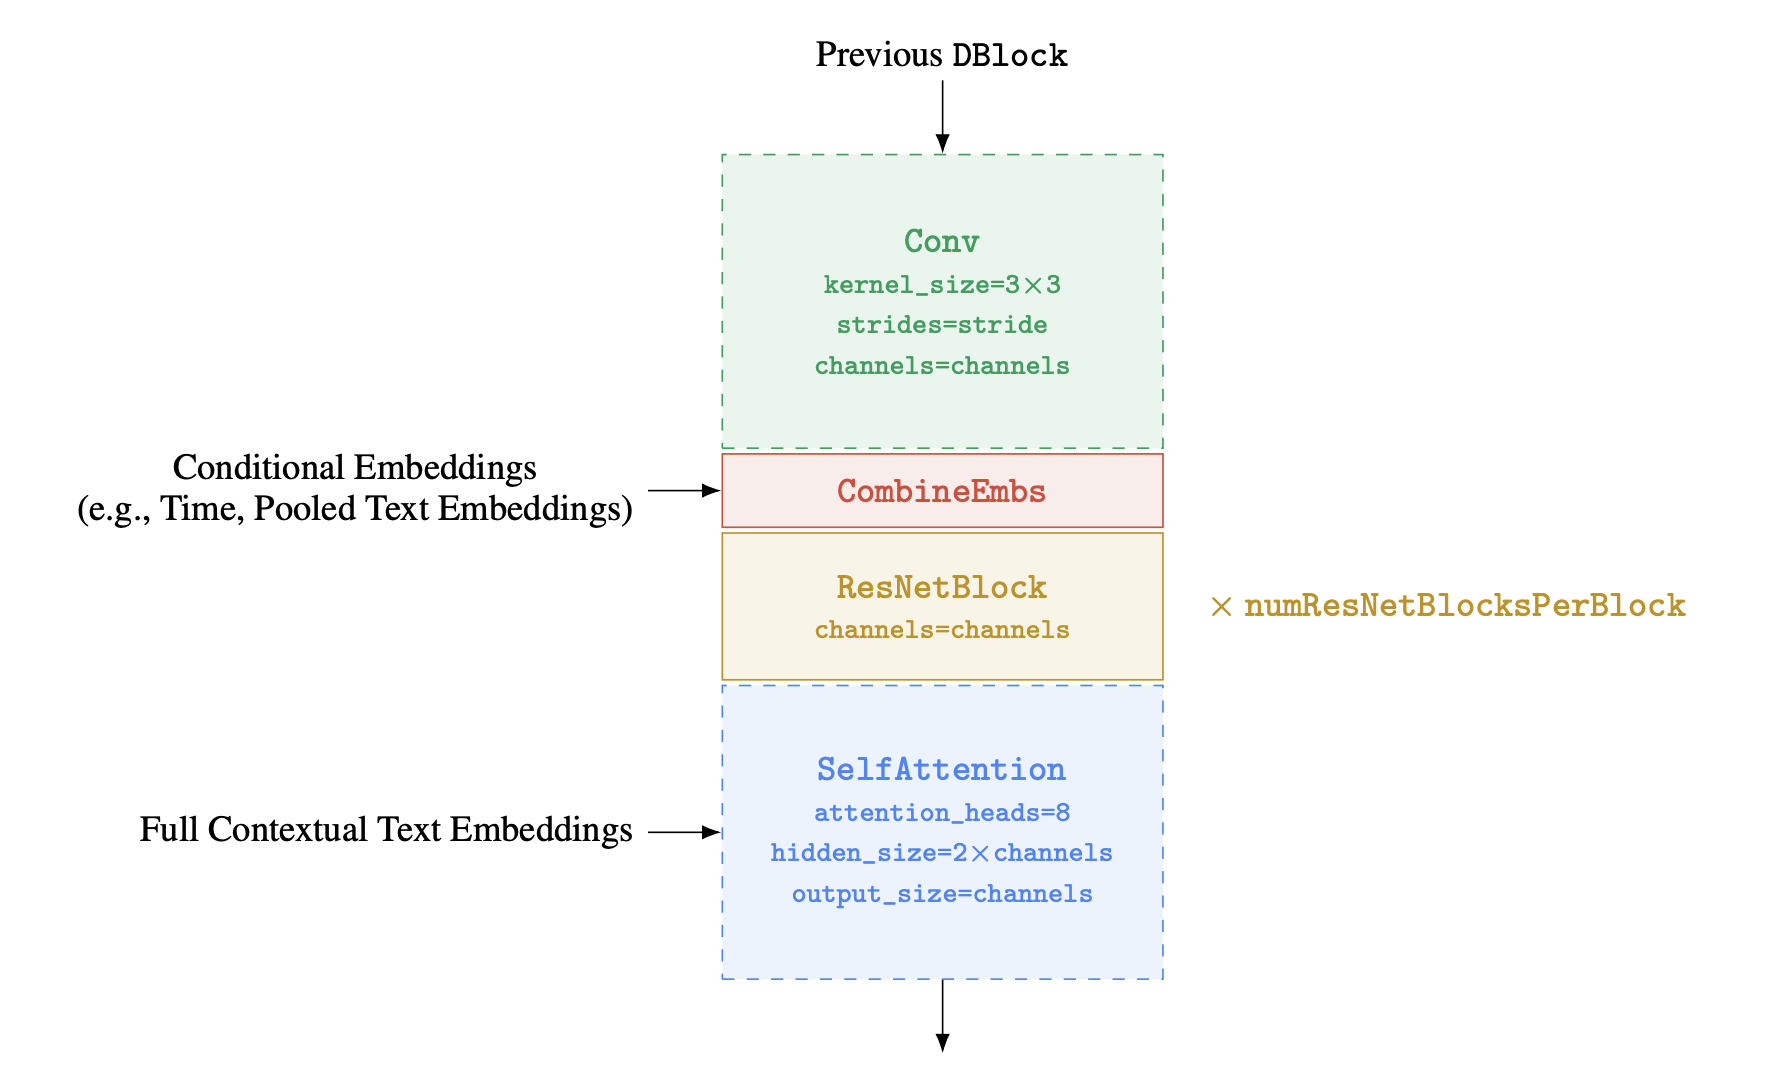
\includegraphics[width=\textwidth]{images/appendix/imagen/dblock.png}
        \caption[]%
        {{\small Imagen efficient U-Net \texttt{DBlock} architecture \cite{imagen}.}}
    \end{subfigure}
    \hfill
    \begin{subfigure}[b]{0.475\textwidth}
        \centering
        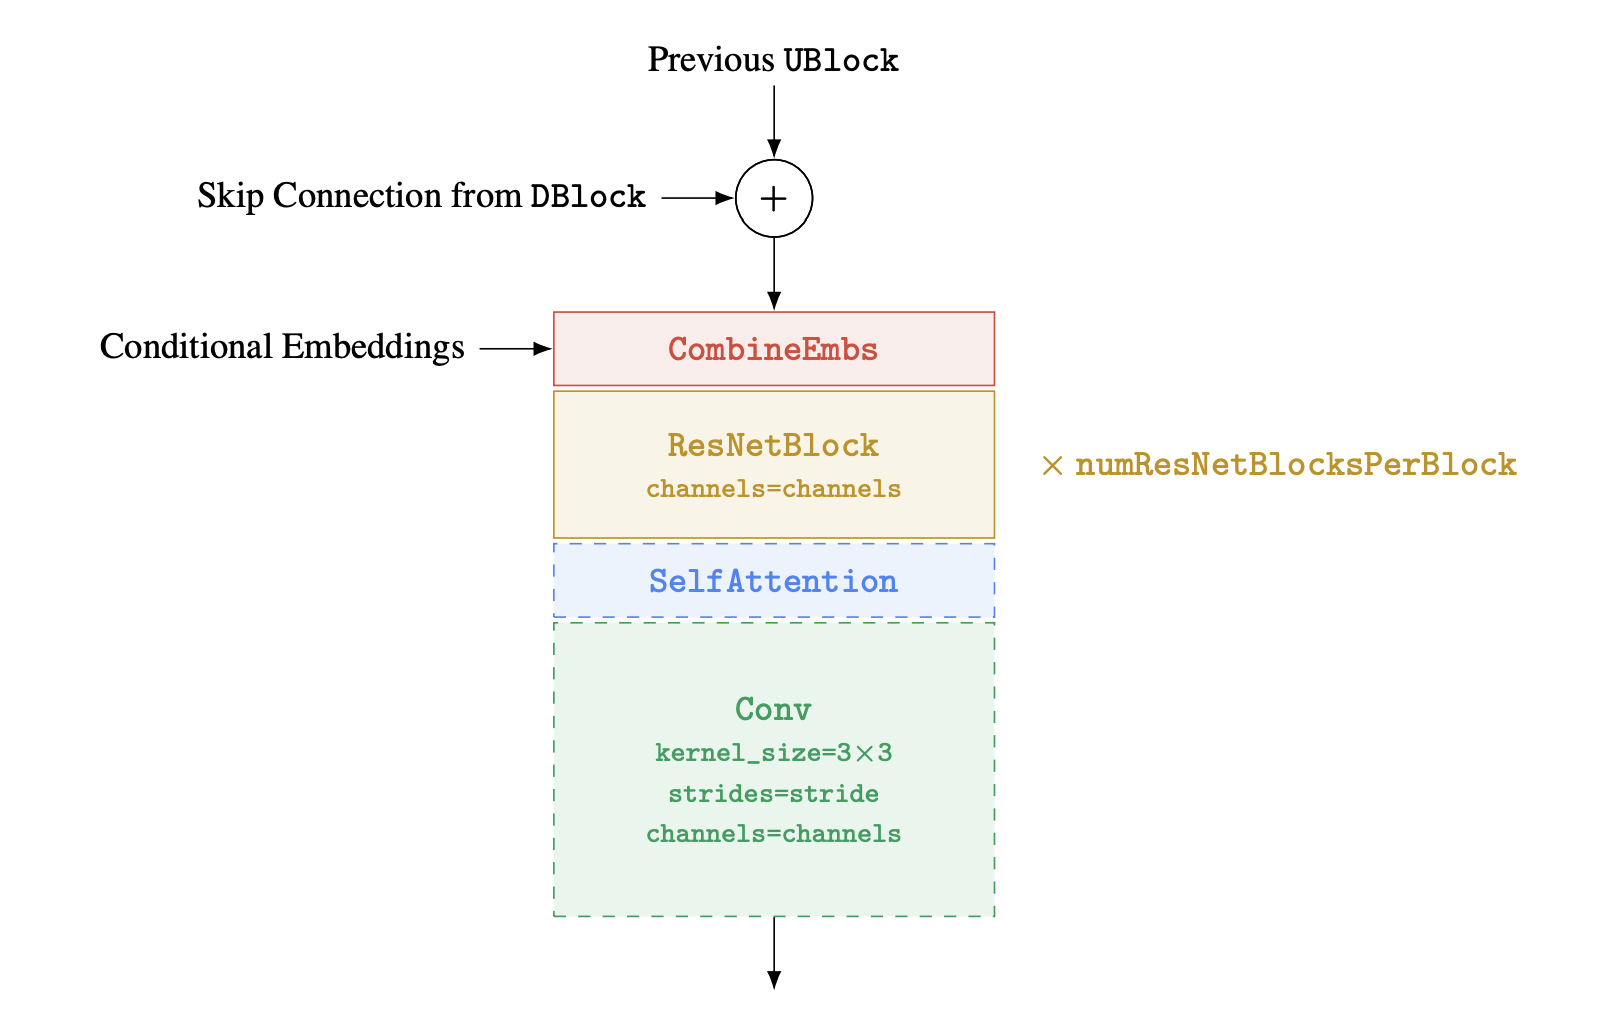
\includegraphics[width=\textwidth]{images/appendix/imagen/ublock.png}
        \caption[]%
        {{\small Imagen efficient U-Net \texttt{UBlock} architecture \cite{imagen}.}}
    \end{subfigure}
\end{figure*}















\subsection{DrawBench}

The COCO dataset \cite{coco_dataset} is a standard benchmark for evaluating T2I models. The standard performance metrics used are FID \cite{fid_score} which measure image fidelity (but is not fully aligned with perceptual quality \cite{perceptual_quality}), and CLIP score \cite{openai_clip} which measures image-text alignment (but is bad at counting objects in an image).

Due to these limitations, the researchers created new benchmark called \textbf{DrawBench} that uses human evaluation to assess image quality by asking "Which image is more photorealistic (looks more real)?" and text-image alignment by asking "Does the caption accurately describe the above image?". For both cases they used 200 randomly chosen image-caption pairs from COCO dataset.

\begin{figure}
    \centering
    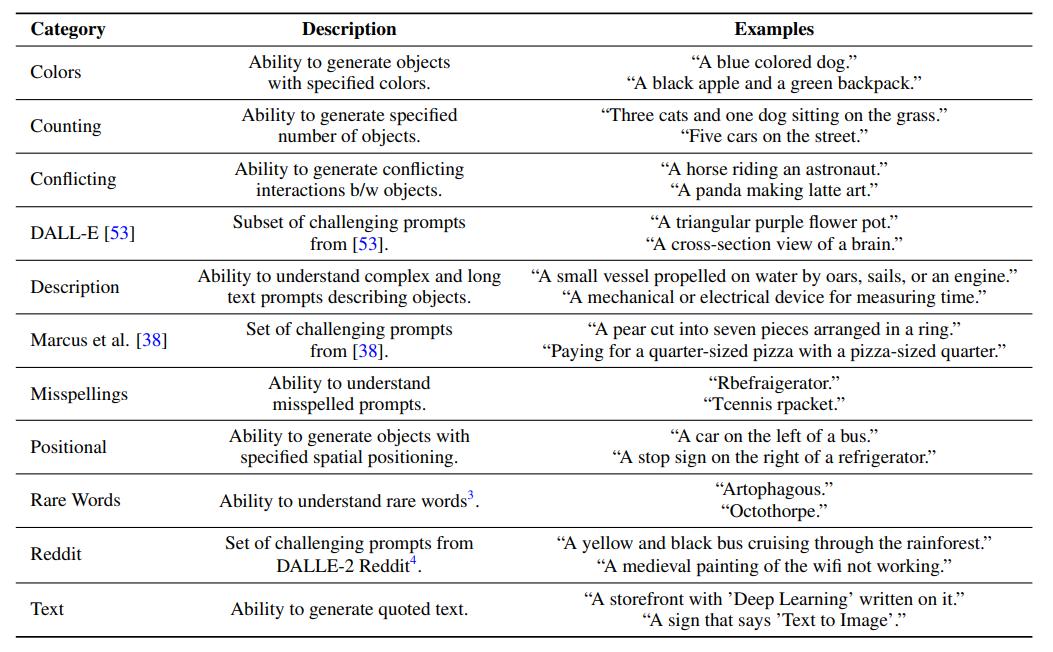
\includegraphics[width=0.6\textwidth]{images/imagen/drawbench_categories.png}
    \caption{Descriptions and examples of the 11 categories in DrawBench \cite{imagen}.}
    \label{fig:imagen_drawbench_categories}
\end{figure}

DrawBench has 11 categories of prompts which test different capabilities of models such as ability to render different colors, number of objects, spatial relations, text in the scene, and more. The prompts include long captions, rare words, and misspelled prompts. See figure \ref{fig:imagen_drawbench_categories} for examples of the categories and examples.














\subsection{Results}

\begin{figure}[t!]
    \centering
    \begin{subfigure}{0.4\textwidth}
        \centering
        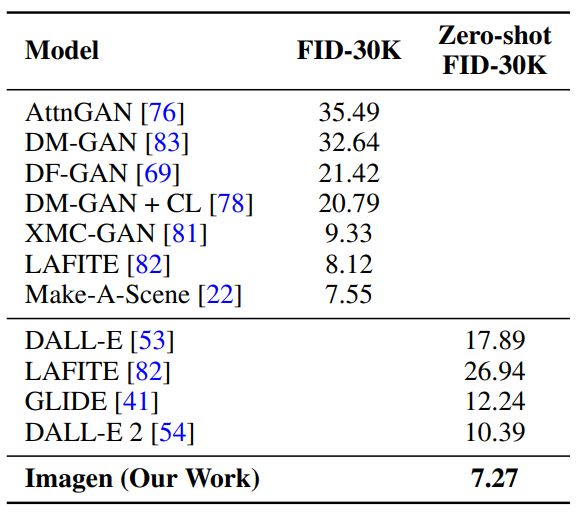
\includegraphics[width=0.6\linewidth]{images/imagen/imagen_coco_zeroshot.png}
        \caption{Although Imagen was not explicitly trained on MS-COCO dataset, it outperforms all other models on COCO FID score, achieving 7.27 FID.}
        \label{fig:imagen_coco_zeroshot}
    \end{subfigure}
    \begin{subfigure}{0.4\textwidth}
        \centering
        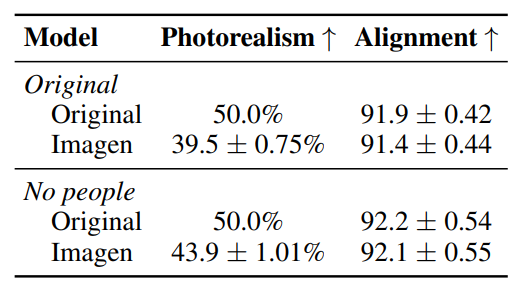
\includegraphics[width=0.6\linewidth]{images/imagen/imagen_coco_human_eval.png}
        \caption{Human evaluation on 256x256 COCO. Imagen splits to two categories: no filters, and human filters. Imagen struggles a little with photorealistic people.}
        \label{fig:imagen_coco_human_eval}
    \end{subfigure}
    \caption{Results of Imagen on COCO dataset \cite{imagen}.}
\end{figure}

\begin{figure}
    \centering
    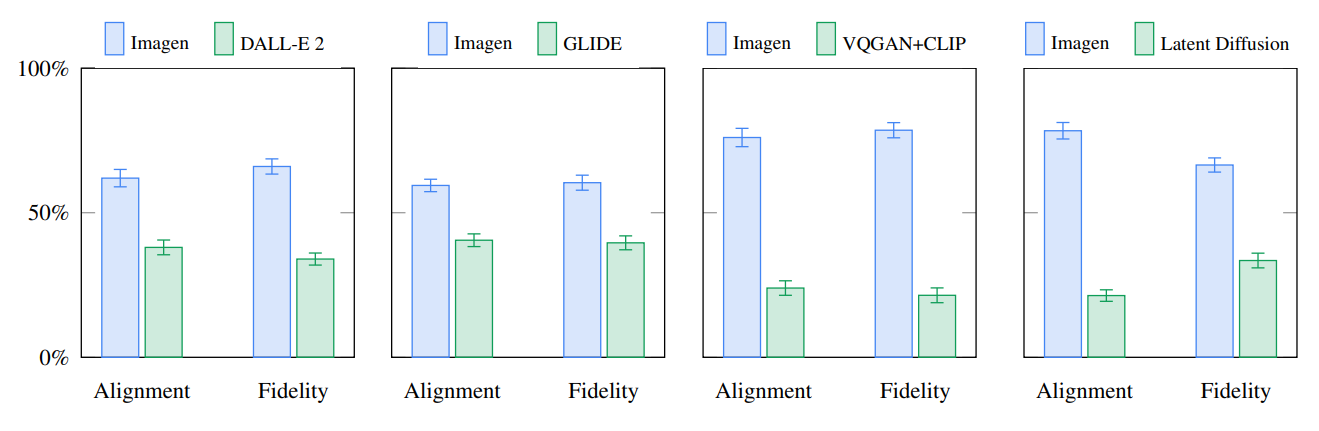
\includegraphics[width=0.6\textwidth]{images/imagen/alignment_fidelity_imagen_vs_models.png}
    \caption{Imagen beats all other models (DALL-E 2 \cite{dalle_2}, GLIDE \cite{glide}, VQ-GAN+CLIP \cite{vqgan_clip} and Latent Diffusion (Stable Diffusion) \cite{stable_diffusion} (section \ref{sec:stable_diffusion})) in terms of image-text alignment and image fidelity \cite{imagen}.}
    \label{fig:imagen_alignment_fidelity_vs_other_models}
\end{figure}

In figure \ref{fig:imagen_coco_zeroshot} we can see that although Imagen was not trained on the MS-COCO dataset, it still outperforms state-of-the-art models such as DALL-E 2 \cite{dalle_2} and achieves the best MS-COCO FID score of 7.27 in zero-shot setting.

In figure \ref{fig:imagen_coco_human_eval} we can see that Imagen achieves a respectable 43.9\% fool rate on $256\times 256$ COCO human faces, indicating limited ability of Imagen to generate photorealistic people.

And in figure \ref{fig:imagen_alignment_fidelity_vs_other_models} we can see that Imagen outperforms all other state-of-the-art models in terms of image fidelity and text-image alignment.
